%%%%%%%%%%%%%%%%%%%%%%%%%%%%%%%%%%%%%%%%%%%%%%%%%%%%%%%%%%%%%%%%%%%
% Background
% Team:
% Wolverine
% Members: 
% Eric Lee, Jacky Wu, Karthick Mani, 
% Eric Chang, Dexter Chen, Peter Chen
% Relative files:
% Background_Wolverine.tex, Library.bib, WolverineChart.png
% Note: 
% Do not compile this file compile Main.tex to get the pdf file instead.
%%%%%%%%%%%%%%%%%%%%%%%%%%%%%%%%%%%%%%%%%%%%%%%%%%%%%%%%%%%%%%%%%%%
	
\subsection{Information retrieval on existing database}
\textit{\footnotesize Author:Dexter Chen, Eric Chang, Eric Lee, Jacky Wu,\\ 
	Karthick Mani, Kenvin Lo, Yu-cheng Chen.}\\

We live in the time where technologies evolve beyond our imagination. Due to the rapidly increasing amount of information, we can't rely on the old fashion ways to find data. We need new information retrieval methods to handle such a big amount of data. But most of the information retrieval methods such as search engine can't really search everything on the web. They can only search the data that has been captured into the database according to \cite{Grehan}. Thus, we need to create a database to store these data and automatically update them frequently.

There are several online libraries currently available for us to get the academic articles we need. And they can be roughly divided into three group according to the way they store articles.
\subsubsection*{Index libraries}	
	These kind of libraries store the index and abstract of the articles. They don't provide the full text documents directly, but may give the linkage to the publisher websites of articles. And can be categorize by the type of articles they include.
	\begin{itemize}
		\item\textbf{Comprehensive topics}\\Libraries such as Web of Science, Scopus...
		\item\textbf{Specialized topics}\\Libraries such as Compendex, BIOSIS Previews, PubMed...
	\end{itemize}
\subsubsection*{Publisher libraries}
	These libraries are created by the publishers themselves, so they provide the newest and complete documents directly. And can also be categorize by the type of articles they include.
	\begin{itemize}
		\item\textbf{Comprehensive topics}\\Libraries such as Science Direct, Springer Link, Wiley Online Library...
		\item\textbf{Specialized topics}\\Libraries such as Nature.com, Emerald Management Xtra, IEEE Xplore...
	\end{itemize}
\subsubsection*{Aggregator libraries}
	These libraries do not published the articles by themselves, but they still sometimes provide the full text articles to the user. The way they do this is to negotiate with some of the publisher libraries and get the authorization of the articles. Libraries such as EBSCOhost, ProQuest, JSTOR...

\subsubsection*{Introduction of several publisher libraries }
With the knowledge we gained  through this study will be utilized to create a data base for open access full-text articles. The publisher library should be focused on this study as these kind of library have their own data base to store full-text articles in PDF. In the following paragraph, this study will go to introduce several popular publisher libraries and discuss how they store full-text articles in PDF.
\begin{enumerate}
	\item {Science Direct}
	\item {Springer Link}
	\item {IEEE Xplore}
\end{enumerate}

\begin{figure*}[htb]
	%\begin{wrapfigure}{i}{\textwidth}
	\begin{center}
		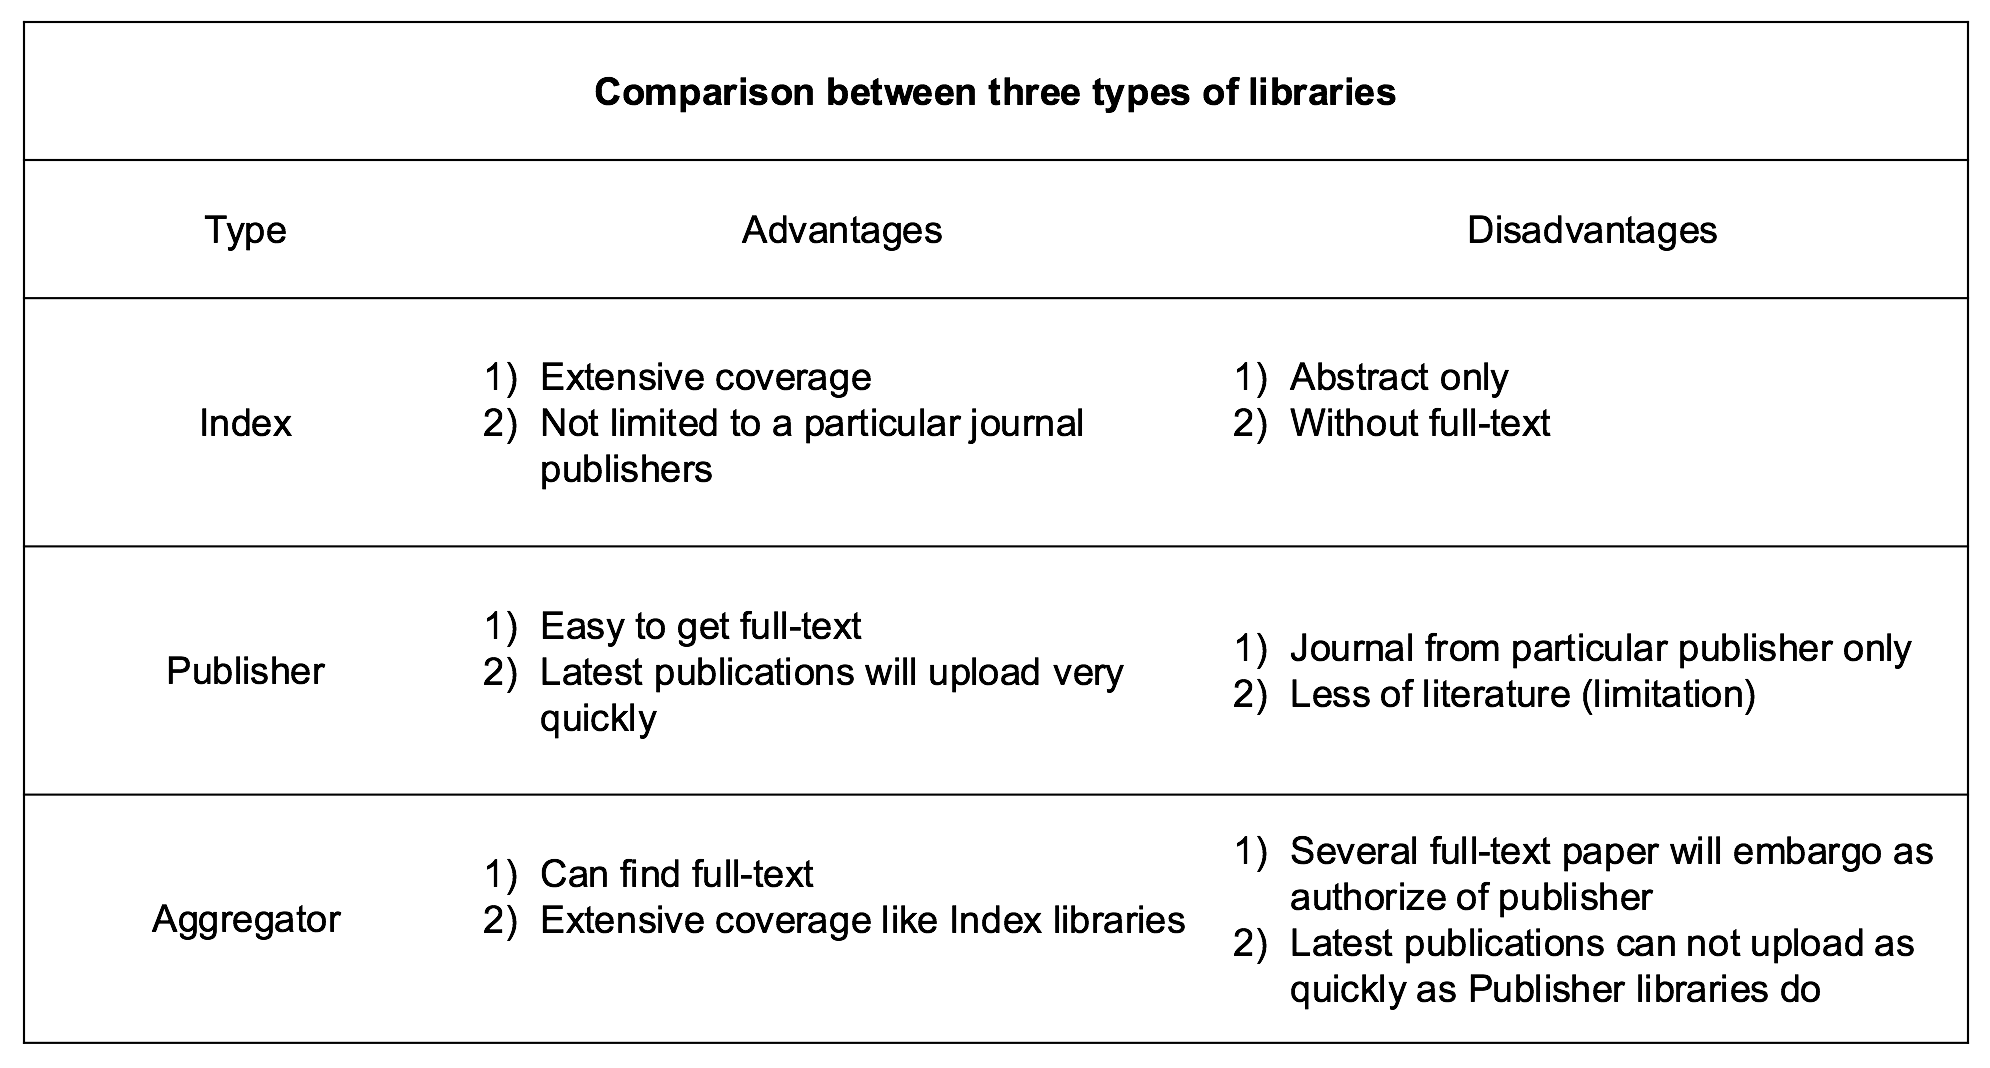
\includegraphics[width=0.8\textwidth]{WolverineChart3}
	\end{center}
	\caption{Comparison between three types of libraries}
	%\end{wrapfigure}
\end{figure*}
\clearpage
